% LEXICAL STRESS ERRORS
%
% !TEX root = ../thesis-main.tex
%
%TODO change title? \chapter{Lexical stress errors in the IFCASL corpus}
\chapter{Lexical stress errors by French learners of German \TODO{title?}}
\label{chap:lexstress}

%\cleanchapterquote{You can’t do better design with a computer, but you can speed up your work enormously.}{Wim Crouwel}{(Graphic designer and typographer)}

%\blindtext

%\section{Stress in German vs. French }
%	\subsection{Comparative prosody}
%	\subsection{Stress ``deafness'' in French}
%	\subsection{Expected errors}
%	
	
\TODO{Change title?}
%\section{Lexical stress errors in the IFCASL corpus} 

	\TODO{Reminder of IFCASL corpus} see \cref{sec:intro:ifcasl}

	To investigate to what extent the expected lexical stress errors by French speakers of German are actually produced, a subset of the non-native German-language IFCASL corpus was annotated for such errors, with a view to answering the following questions:

	\TODO{Put questions in same order as results subsections}
	\begin{itemize}
	\item{Are lexical stress errors observed frequently in the IFCASL data?}
	\item{Is there a difference in the frequency of these errors among different groups of speakers (i.e. in terms of skill level, age, or gender) or in different contexts (e.g. after hearing a native speaker produce the word)?}
	\item{Are lexical stress errors observed more frequently with certain word types than with others?}
	\item{Can lexical stress errors be reliably identified by native German speakers (i.e. to what extent do the judgments of different annotators agree)?}
	\item{Are there differences in how expert and novice annotators (those without annotation experience or any training in phonetics/phonology) identify lexical stress errors?} 
	\item{Are there differences in how native and non-native German speakers identify errors?}
	\item{How frequently do technical problems interfere with determining the accuracy of a production?}
	\end{itemize}
	
	This chapter describes the annotation of this sub-corpus, and presents an analysis of the annotated data that provides tentative answers to the above questions. \TODO{rephrase that?}
	%This chapter presents the data and method used for this annotation, and an analysis of the annotated sub-corpus \TODO{\textit{rephrase}: in light of these guiding questions}. 
	
	%\subsection{Data}
	\section{Data}
	\label{sec:lexstress:data}
	
	The IFCASL sub-corpus annotated for lexical stress errors consists of utterances of twelve word types (see \cref{tab:bisyllwords}), each of which is bisyllabic and canonically has its primary stress on the initial syllable. These characteristics were chosen deliberately: the selected words are bisyllabic because this simplifies comparison between stressed and unstressed syllables, and they are initial-stress because this is the stress pattern which native (L1) French speakers are expected to have the most difficulty producing in German, given the fixed final-position stress and final lengthening in French (see \cref{sec:stress:expected}). 
	
	In the IFCASL corpus recordings, sentences containing these words were read aloud by L1 and L2 (L1 French) speakers. Here, only the L2 utterances were annotated; it is assumed that the L1 German speakers always realize lexical stress correctly. \TODO{justify that assumption?}
	
	As described in \cref{sec:intro:ifcasl} \TODO{verify that this reference is appropriate}, the IFCASL recordings were performed under two conditions: the ``Sentence Read'' (SR) condition, in which the L2 speaker is simply  presented with the text of the sentence and asked to record themselves reading it aloud, and the ``Sentence Heard'' (SH) condition, in which the L2 speaker is asked to listen to an utterance of the sentence by an L1 German speaker before recording their own utterance. The sub-corpus for annotation includes recordings from both conditions, though the majority are from the SR condition \TODO{does mentioning that help or hurt?}.
	
	To compile the sub-corpus for annotation, utterances (tokens) of each word as produced by over 50 L2 speakers were extracted from the recordings automatically in Praat \parencite{Boersma2014}, using the word-level segmentation of each sentence utterance automatically obtained by forced alignment (see \TODO{ref}).
	\TODO{How many tokens couldn't be annotated because of disfluencies, this is a problem that a real CAPT system would have to cope with (reference appropriate section)}
	
	\begin{table}[htb]
		\centering
		\caption{The twelve bisyllabic initial-stress words types selected from the IFCASL corpus for stress error annotation \TODO{column details}%, and the number of distinct tokens annotated (each produced by a different speaker)
		}
%		\begin{tabular}{llll}
%		Flagge & Ringen & Tschechen & halten \\
%		M\"{o}rder & Tatort & Fr\"{u}hling & fliegen \\
%		Pollen & manche & E-mail & tragen \\
%		\end{tabular}
		
		\begin{tabularx}{\textwidth}{lXXXXX}
		\toprule
		
		Orthography & 
		Canonical \linebreak pronunciation & 
		Part of speech & 
		English \linebreak translation & 
		Recording condition & 
		Number \linebreak of tokens \\%\linebreak annotated\\
		
		\midrule
		E-mail	&	\TODO{prons} &	noun &	e-mail &	SR 	&	56	\\
		Flagge	&	&	noun &	 flag &	SH	&	55	\\
		fliegen	&	&	verb &	fly &	SR		& 56	\\
		Frühling	&	& noun	&	spring &	SR		&	56	\\
		halten	&	&	verb &	hold &	SR 	&	56	\\
		manche	&	&	pronoun &	some & 	SR 	&	56	\\
		Mörder	&	&	noun &	murderer &	SR 	&	56	\\
		Pollen	&	&	noun &	pollen &	SR 	& 	55	\\
		Ringen	&	&	noun &	rings &	SH	&	55	\\
		Tatort	&	&	noun &	crime scene & 	SR 	&		56	\\
		tragen	&	&	verb &	wear &	SH	&	55	\\
		Tschechen	&	& noun	&	Czechs	&	SR		& 56	\\
		\bottomrule
		\end{tabularx}
		\label{tab:bisyllwords}
	\end{table}
	
	\section{Annotators}
	\label{sec:lexstress:annotators}
	
	A total of 15 annotators participated in the annotation of this IFCASL sub-corpus \TODO{\textit{remove?:} over the course of 2 months}, each of whom is listed in \cref{tab:annotators} (by an arbitrary identifier, to preserve anonymity).
	As \cref{tab:annotators} shows, the annotators varied with respect to their native language, as well as with respect to their level of expertise in phonetics/phonology/linguistic annotation. 
	 
	 % Nativeness
	Of the 15 annotators, the majority (12) were native German speakers, two were native speakers of American English, and one annotator's first language was Hebrew. The nonnative speakers all have \TODO{\textit{more specific?:} some knowledge}  of German as L2.
	%
	% Expertise
	In terms of expertise, the annotators can broadly be categorized into three groups: 
	\begin{itemize}
	\item{\textit{expert} annotators are professional researchers with a thorough understanding of phonetics/phonology and extensive experience in annotating speech data}
	\item{\textit{intermediate} annotators are university students \TODO{ enrolled in an experimental phonology course \textit{is that true of Frankfurt students too?}}, and have some training in phonetics/phonology and/or experience annotating speech data}
	\item{\textit{novice} annotators have negligible training in phonetics/phonology and lack experience annotating speech data}
	\end{itemize}
	As shown in \cref{tab:annotators}, the majority of annotators (10 out of 15) fall into the \textit{intermediate} group; two annotators can be considered \textit{expert}, and there are three \textit{novice} annotators.
	
	\begin{table}[htb]
		\centering
		\caption{Annotators \TODO{caption}}
		
		\begin{tabularx}{\textwidth}{lllX}
		\toprule
		ID & Native language & Expertise & Word types annotated (number of tokens) \newline \TODO{alphabetize}\\
		\midrule
		%Frank	FZ 
		A	&	German	& expert & Flagge (55),  Ringen (55), Tschechen (56) \\
		
		%Raphael	RM	
		B	&	German	& intermediate & 	halten (56),  M\"{o}rder (56),     Tatort (56) \\
		
		%Lukas	LS	
		%C & German & intermediate &		Fr\"{u}hling (0), fliegen (0),  Pollen (0) \TODO{Remove entirely?}  \\
		
		%Tobias	TB	
		%P
		C & German & novice & 	halten (56),  Pollen (55),  E-mail (56)	 \\
		
		%Diana	DA 
		D &	German & intermediate &		Pollen (53), Flagge (49),  Ringen (49)	 %\TODO{FALSE}   
		\\
		
		%Patrick	PC 
		E & English (US)	& intermediate & 	Tschechen (56),  halten (56),  M\"{o}rder (56) 	 \\
		
		%Sarah	SC
		F & 	German	 & intermediate & 	Tatort (56), Fr\"{u}hling (56), fliegen (56)	 \\
		
		%Yoav	YB	 
		G & Hebrew	& intermediate & 	fliegen (0),  Pollen (0), Flagge (20)	 %\TODO{FALSE}   
		\\
		
		%Jeanin	JJ	
		H & German & expert &		Fr\"{u}hling (56), fliegen (56),  Pollen (55) \\
		
		%Dilber	DB 
		J & 	German & intermediate &		Ringen (55), Tschechen (56), halten (56)	 \\
		
		%Christine	CM
		K &	German	 & intermediate & M\"{o}rder (56),    Tatort (56), Fr\"{u}hling (56) \\
		
		%Anjana	AV	
		L & English (US)	& intermediate &  manche (56),   E-mail (56),   tragen (55),	    fliegen (56),  Pollen (55), Flagge (55) \\
		
		%Marc	MS	
		M & German	 & novice & Flagge (54), \TODO{mention?}  Tatort (56),  E-mail (56) 	 \\
		
		%Maya	ML
		N & 	German	 & intermediate & Ringen (54), \TODO{mention?}  Fr\"{u}hling (56), tragen (55)	 \\
		
		%Lisa	LB	
		O & German	& novice & Tschechen (56),  fliegen (56),  manche (56)	 \\
		
		%Steffen	SB
		%Q
		P	& German	 & intermediate & Mörder (56),   manche (56),  tragen (55) \\
		
		\bottomrule
		\end{tabularx}
		\label{tab:annotators}
	\end{table}
	
	Each annotator was assigned three word types to annotate in a single session, with the exception of one annotator who was assigned six word types over two sessions (see \cref{sec:lexstress:method} for a description of an annotation session). \Cref{tab:annotators} lists the word types assigned to each annotator, along with the number of tokens labeled for each type. Some judgments by annotators \TODO{D and G} had to be excluded from the analysis due to technical problems; the token counts for each annotator in \cref{tab:annotators} reflect only their usable judgments. \TODO{move following to agreement section in results?} Word types were assigned such that each word type was annotated by at least two native German speakers, and to maximize the amount of overlap between annotators in order to obtain as many pairwise measures of annotator agreement as possible; \cref{tab:annotatorsbyword} lists the number of annotators for each word type.
	
	
	\begin{table}[htb]
		\centering
		\caption{Number of annotators by word type}
		\begin{tabular}{lccc}
		\toprule
		Word type 
		&		Native %annotators 
		& 	Nonnative %annotators 
		& Total %annotators 
		\\
		\midrule
		E-mail	& 2 &	1 &	3 \\
		Flagge	& 3	& 2	& 5 \\
		fliegen	& 3	& 1	& 4 \\
		Frühling	& 4	& 0	& 4 \\
		halten	& 3	& 1	& 4 \\
		manche	& 2	& 1	& 3 \\
		Mörder & 	3	& 1	& 4 \\
		Pollen	& 3	& 1	& 4 \\
		Ringen	& 4	& 0	& 4 \\
		Tatort	& 4	& 0	& 4 \\
		tragen	& 2	& 1	& 3 \\
		Tschechen 	& 3	& 1	& 4 \\
		\bottomrule
		\end{tabular}
		\label{tab:annotatorsbyword}
	\end{table}
	
	
	%\subsection{Annotation method}
	\section{Annotation method}
	\label{sec:lexstress:method}

	The annotation task consisted of assigning one of the following labels to 
	%the lexical stress realization in 
	each token of the selected word types, i.e. each utterance of each word by each L1 French speaker in the corpus:
	
	\TODO{decide on format for labels (\textbf{[this]}?)}
	\begin{itemize}
	\item{\textbf{correct}: the speaker audibly stressed the lexically stressed (initial) syllable}
	\item{\textbf{incorrect}:the speaker audibly stressed the lexically unstressed (final) syllable}
	\item{\textbf{none}: the speaker did not clearly stress either syllable, i.e. did not audibly differentiate stressed and unstressed syllables, or the annotator was unable to determine which syllable was stressed}
	\item{\textbf{bad\_nsylls}: the speaker pronounced the word with an incorrect number of syllables (i.e. by inserting or deleting a syllable), rendering it impossible to judge whether stress was realized correctly or not}
	\item{\textbf{bad\_audio}: a problem with the audio file (e.g. noise in the signal or very inaccurate segmentation) interfered with the annotator's ability to judge the stress realization}
	 \end{itemize}
	
	Annotation proceeded by means of a graphical tool scripted in Praat \parencite{Boersma2014}, the main interface of which is shown in \cref{fig:annotationtool}. At the top, a word's text is displayed, along with the IFCASL corpus ID number of the speaker whose utterance of that word will be annotated (this number is only relevant for the annotator insofar as changes in its value inform the annotator that the speaker is changing from utterance to utterance). The recording of the word
%, extracted automatically from the utterance of the entire sentence using the boundaries of the forced-alignment segmentation, 
is played once automatically; the annotator may then choose to click one of the green buttons to play the word again, or play the recording of the entire sentence, as many times as they wish. Once the annotator has judged the accuracy of the lexical stress realization in this utterance, they log that judgment by clicking one of the gray buttons. The annotator is then automatically advanced to the next utterance, with the counts in the lower right corner tracking their progress towards the total number of tokens to be annotated. 

A single annotation session consisted of annotating all tokens of three word types, and lasted approximately 15 minutes. As mentioned in \cref{sec:lexstress:annotators} above, each annotator participated in one session, with the exception of annotator L who participated in two sessions (separated by several days) and annotated a total of six word types.
	
		\begin{figure}[bht]
			\centering
			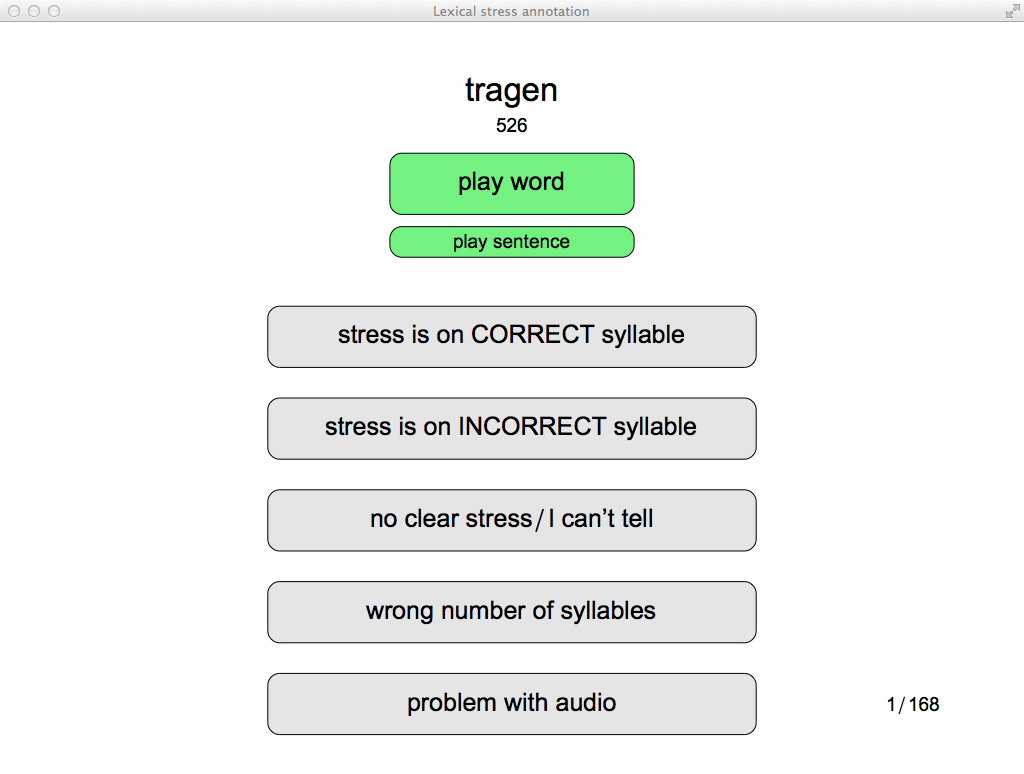
\includegraphics[width=\textwidth]{img/screenshots/AnnotationTool}
			\caption[A screenshot of the graphical annotation tool scripted in Praat.]{A screenshot of the graphical annotation tool scripted in Praat. Green buttons allow the annotator to listen to  the word and sentence utterances. Gray buttons allow the annotator to record their judgment of stress accuracy; from top to bottom, the buttons correspond to the labels [correct], [incorrect], [none], [bad\_nsylls], and [bad\_audio]. \TODO{border around graphic}}
			\label{fig:annotationtool}
		\end{figure}
	
	%\subsection{Results}
	\section{Results}
	\label{sec:lexstress:results}	
	
	\TODO{Intro}
	
	\TODO{Section organization?}
	
		
		
		\subsection{Inter-annotator agreement}
		\label{sec:results:agreement}
		
		\TODO{}
	
	
		\TODO{Explain how a final label was decided for each token}
	
		%\subsubsection{Native vs. nonnative annotators}
		\subsection{Native vs. nonnative annotators}
		\label{sec:results:native}
		
		

		In comparing the relative frequencies of the different response classes, illustrated in \cref{fig:l1pies}, we observe that the native and nonnative speakers judge utterances as having correct lexical stress with approximately the same frequency: 52.7\% of native annotators' judgments are \textbf{[correct]}, vs. 57.3\% for nonnative annotators. However, nonnative speakers seem to choose the \textbf{[none]}
		%``no clear stress/I can't tell'' 
		label somewhat more frequently than native speakers (21.3\% vs. 11\%); this could indicate that nonnative speakers are less confident about how stress should be realized in German, resulting in less certainty about whether a given utterance is correct or not. \TODO{update/verify this paragraph}
		
		
			\begin{figure}[htb]
				\centering
				\begin{subfigure}[b]{.5\textwidth}
					\centering
					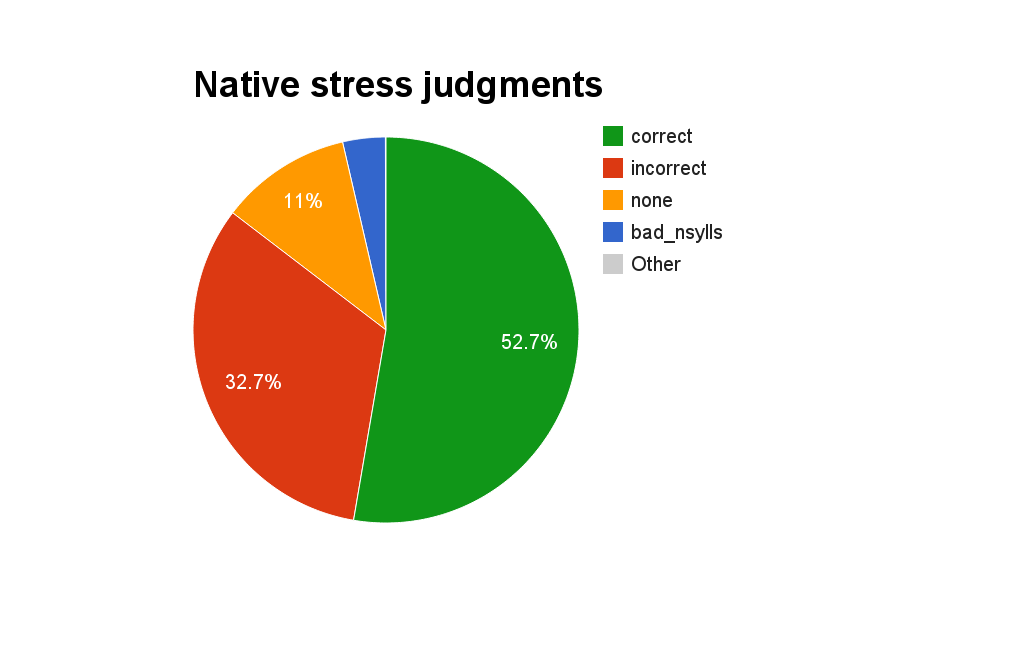
\includegraphics[width=\textwidth]{img/annotation/nativePie}
					\caption{Native annotators}
					\label{fig:l1pies:native}
				\end{subfigure}%
				~
				\begin{subfigure}[b]{.5\textwidth}
					\centering
					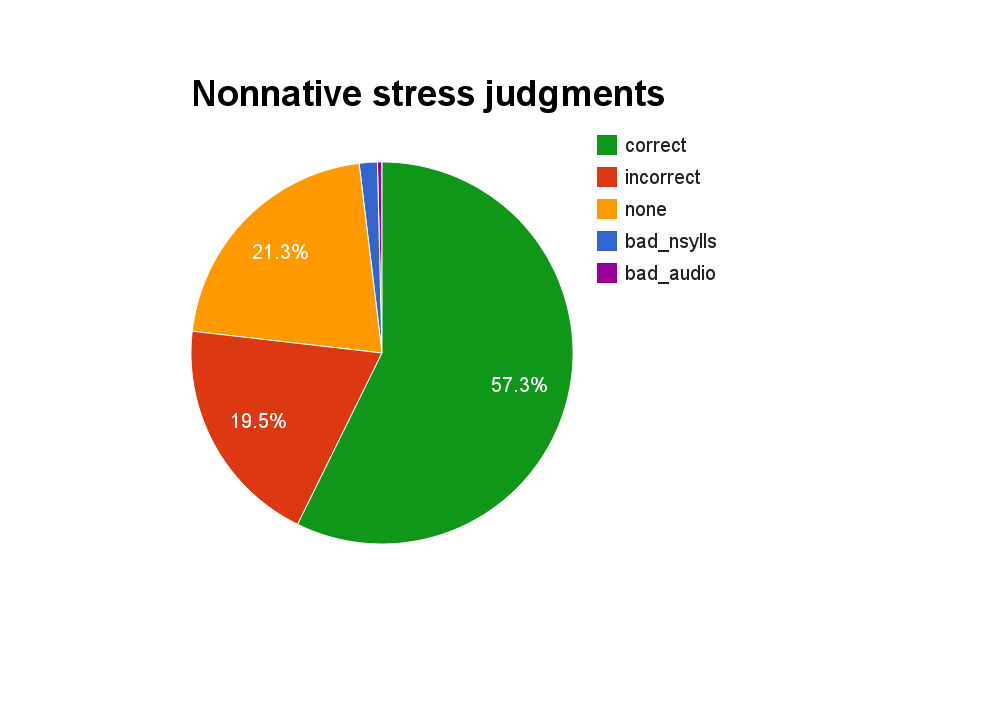
\includegraphics[width=\textwidth]{img/annotation/nonnativePie}
					\caption{Nonnative annotators}
					\label{fig:l1pies:nonnative}
				\end{subfigure}%
				\caption{Stress judgments made by native and nonnative German speakers}
				\label{fig:l1pies}
			\end{figure}
			
		
		\subsection{Expert vs. novice annotators?}
		\label{sec:results:expert}
		
			\Cref{fig:expertisepies} illustrates the relative number of each label type as assigned by annotators of the three expertise levels described in \cref{sec:lexstress:annotators} above, and while any analysis of this data should bear in mind the small sample sizes of the expert and novice groups (two and three annotators, respectively), it does appear that some interesting differences may exist between the three groups. 
			
			Expert annotators seem to be far more ``generous'' in their labeling than intermediate or novice annotators, in that the experts assigned the \textbf{[correct]} label 73.6\% of the time, in contrast with 49.3\% and 54.8\% for the other two groups respectively. \TODO{\textit{person?:} One could} speculate that experts' familiarity with nonnative speech and knowledge of possible inter-speaker variations in lexical stress realization may be the cause for this willingness to ``accept'' a high proportion of utterances as correct. \TODO{too many scare quotes in this paragraph?}
			
			Another interesting difference can be observed between the intermediate and novice annotator groups: compared with the intermediate annotators, novices assign the \textbf{[none]} label less frequently (5.8\% of the time, versus 16.3\% for intermediates) and the \textbf{[bad\_nsylls]} label more frequently (8.4\% of the time, versus 2.1\% for intermediates). Still keeping in mind the discrepancy in sample sizes when comparing 10 intermediate annotators to three novices, \TODO{\textit{person?:} we might} speculate that if experts' extensive experience with nonnative speech could be an explanation for their ``generosity'' with the correct label, novice annotators' lack of experience with nonnative speech could in a similar way make them ``harsher'' in judging nonnative utterances as having an incorrect number of syllables. \TODO{This paragraph sucks. Also too many scare quotes.}
			
			%TODO include?
%			\begin{figure}[htb]
%				\centering
%				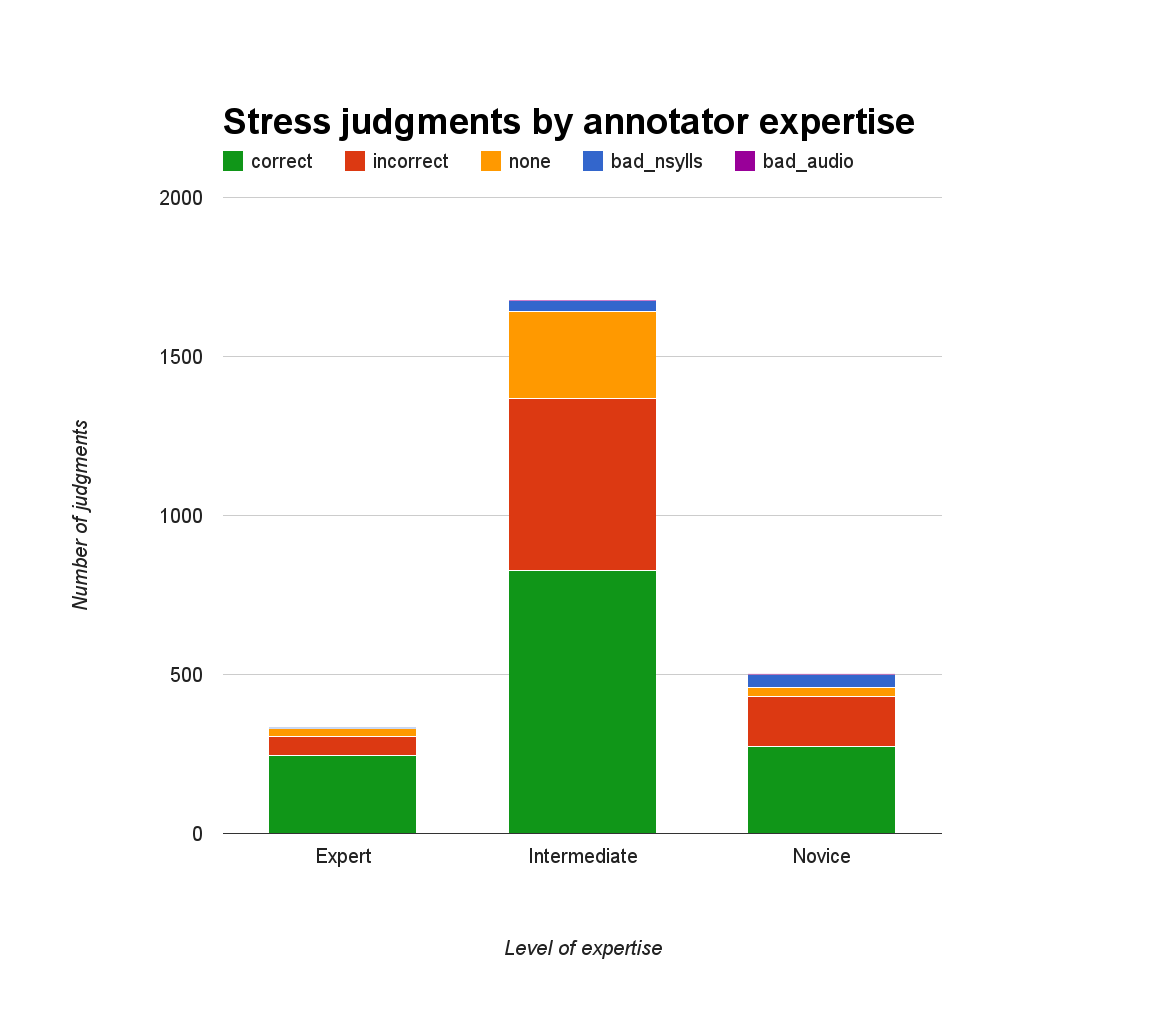
\includegraphics[width=\textwidth]{img/annotation/expertiseBars}
%				\caption{Stress judgments by annotator expertise}
%				\label{fig:expertisebars}
%			\end{figure}
			
			
			\begin{figure}[htb]
				\centering
				\begin{subfigure}[b]{.5\textwidth}
					\centering
					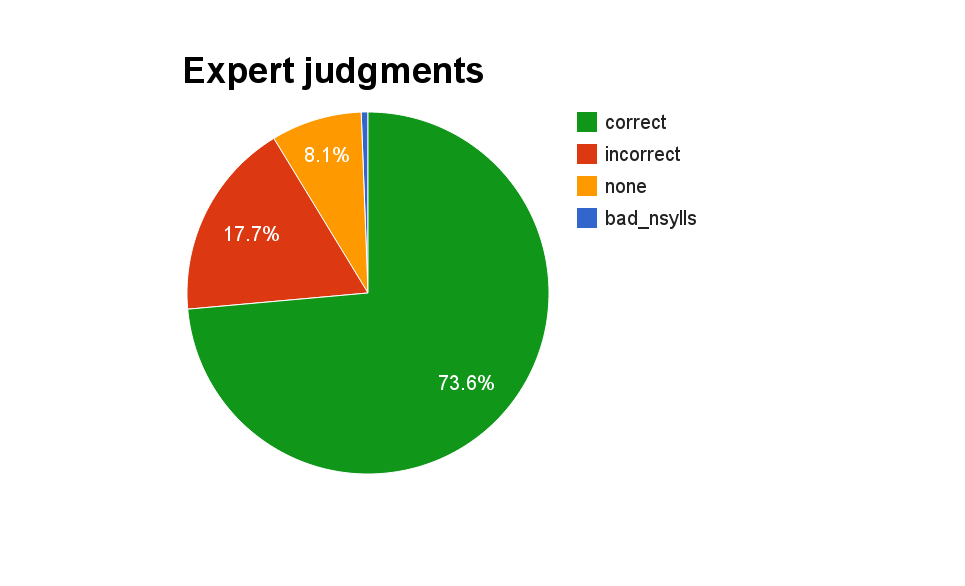
\includegraphics[width=\textwidth]{img/annotation/expertPie}
					\caption{Expert}
					\label{fig:expertisepies:expert}
				\end{subfigure}%
				
				\begin{subfigure}[b]{.5\textwidth}
					\centering
					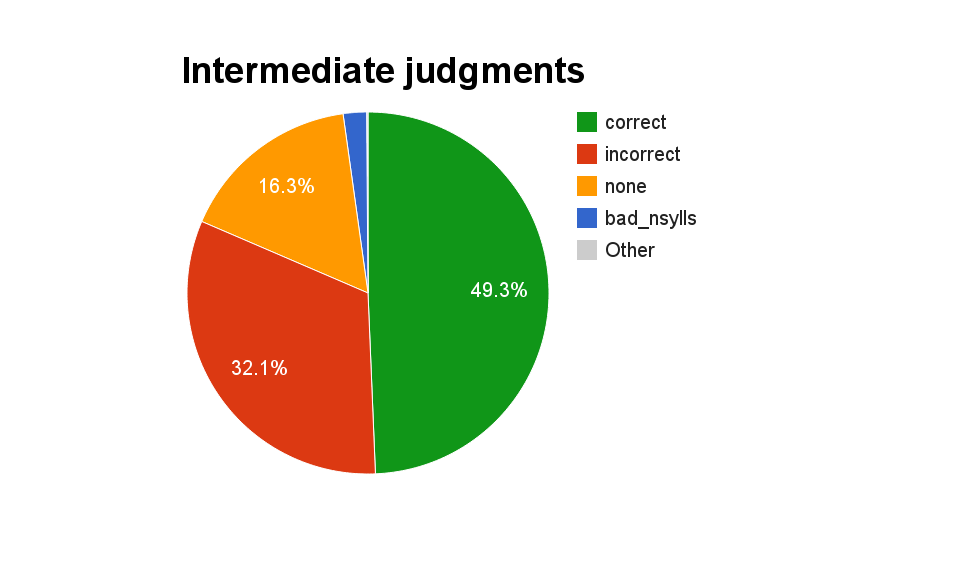
\includegraphics[width=\textwidth]{img/annotation/intermediatePie}
					\caption{Intermediate}
					\label{fig:expertisepies:intermediate}
				\end{subfigure}%
				~
				\begin{subfigure}[b]{.5\textwidth}
					\centering
					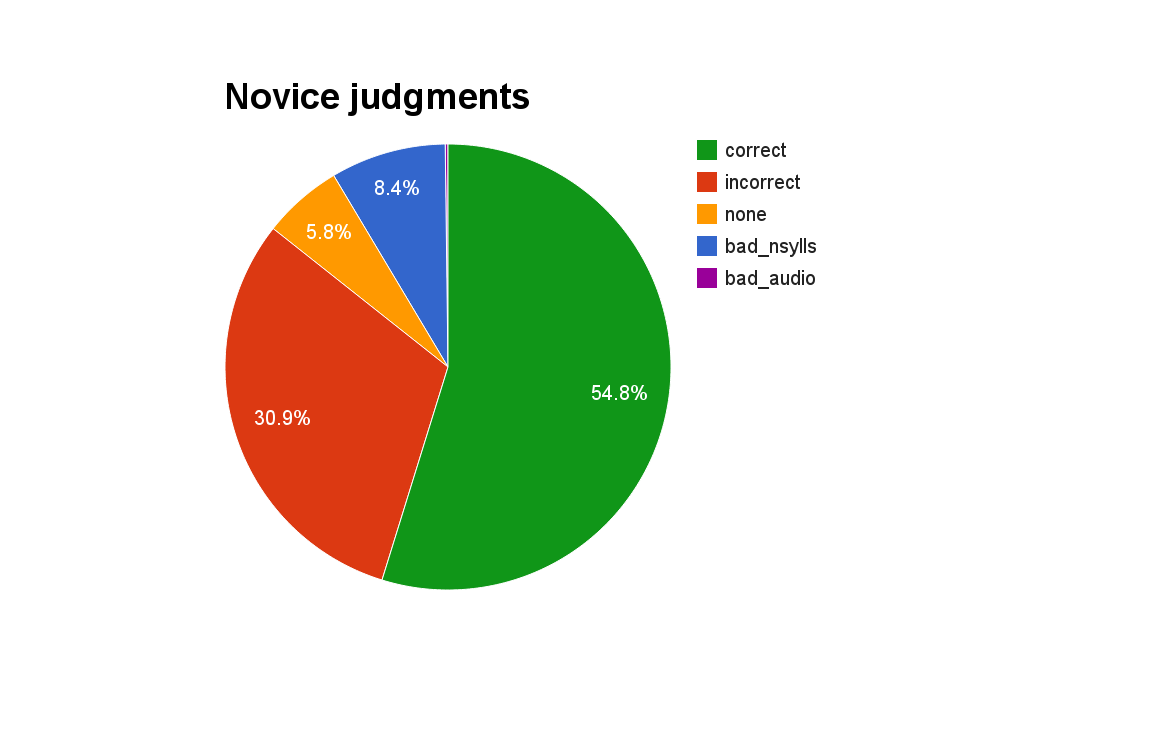
\includegraphics[width=\textwidth]{img/annotation/novicePie}
					\caption{Novice}
					\label{fig:expertisepies:novice}
				\end{subfigure}%
				\caption{Stress judgments by annotator expertise}
				\label{fig:expertisepies}
			\end{figure}
			
			
		\subsection{Overall frequency of lexical stress errors}
		\label{sec:results:overall}
		
		\TODO{Maybe this section should go last instead of first?}
		
		%\subsubsection{Accuracy by L2 skill level}
		\subsection{Errors by L2 skill level}
		\label{sec:results:level}
		
			\TODO{text}
			
			%TODO exclude?
			\begin{figure}[htb]
				\centering
				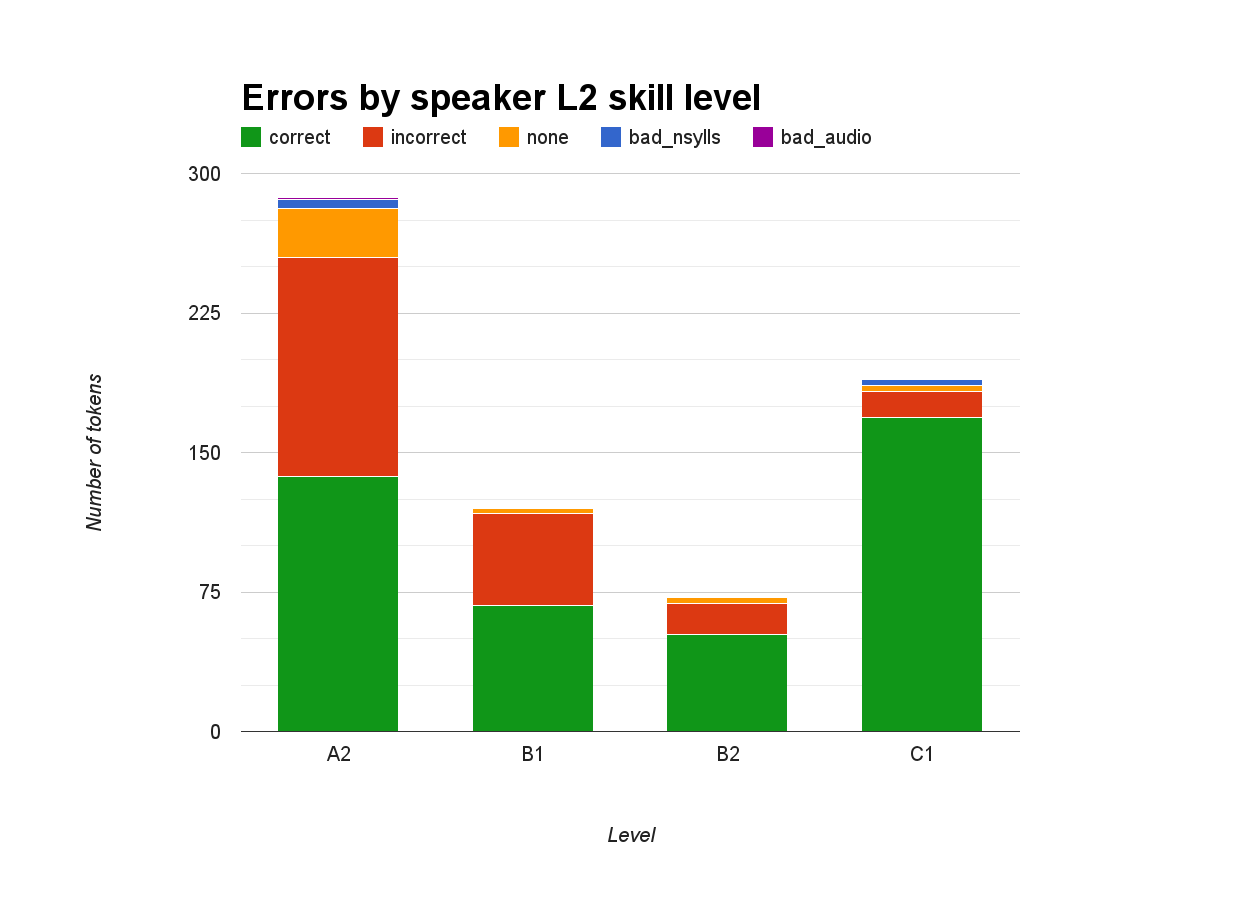
\includegraphics[width=\textwidth]{img/annotation/skillLevelBars}
				\caption{Stress judgments by speaker skill level \TODO{Exclude?}}
				\label{fig:levelbars}
			\end{figure}
		
		
			\begin{figure}[htb]
				\centering
				\begin{subfigure}[t]{0.5\textwidth}
					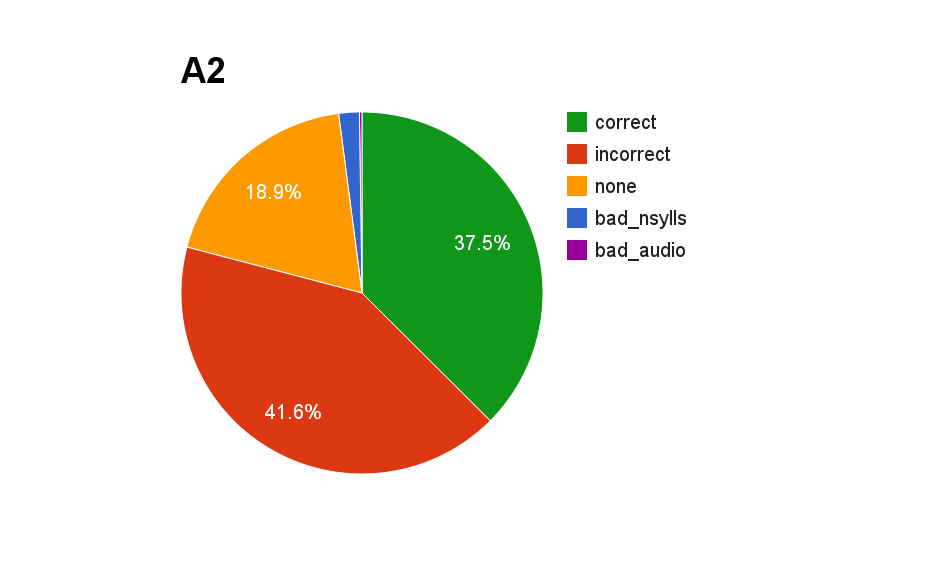
\includegraphics[width=\textwidth]{img/annotation/A2}
					\caption{A2}
					\label{fig:levelpies:A2}
				\end{subfigure}%
				~
				\begin{subfigure}[t]{0.5\textwidth}
					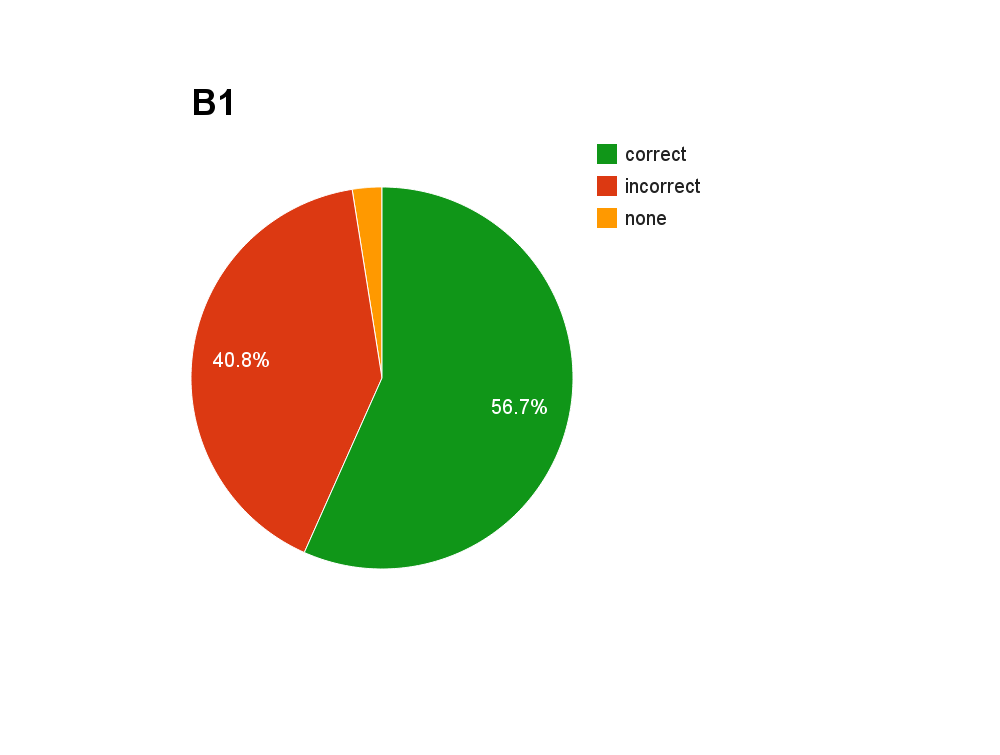
\includegraphics[width=\textwidth]{img/annotation/B1}
					\caption{B1}
					\label{fig:levelpies:B1}
				\end{subfigure}%
				
				\begin{subfigure}[b]{0.5\textwidth}
					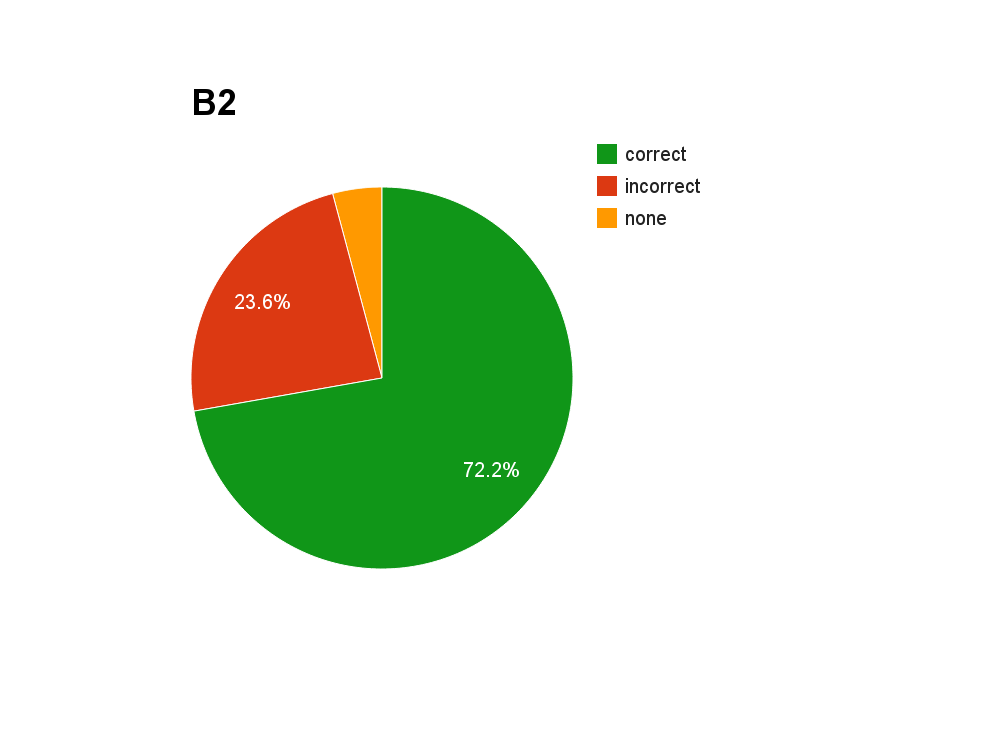
\includegraphics[width=\textwidth]{img/annotation/B2}
					\caption{B2}
					\label{fig:levelpies:B2}
				\end{subfigure}%
				~
				\begin{subfigure}[b]{0.5\textwidth}
					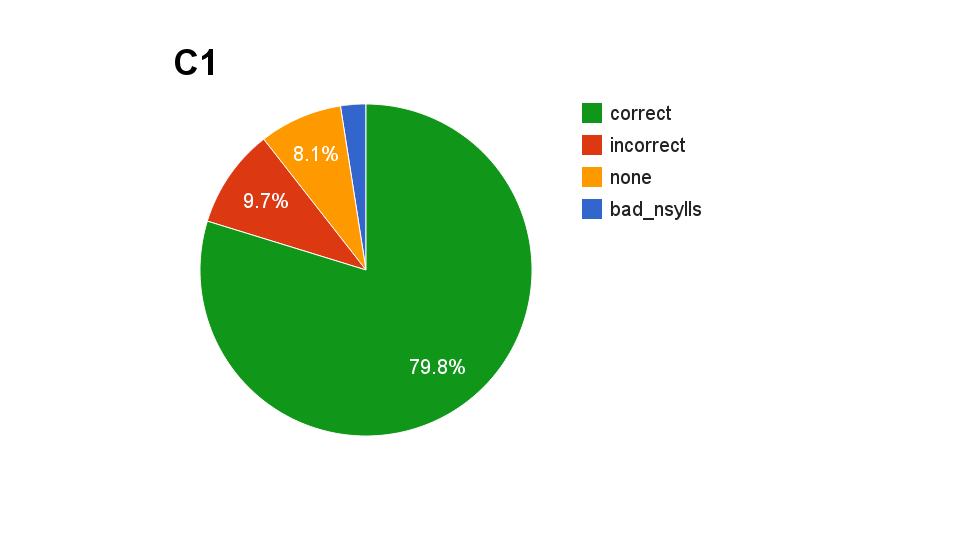
\includegraphics[width=\textwidth]{img/annotation/C1}
					\caption{C1}
					\label{fig:levelpies:C1}
				\end{subfigure}%
				\caption{\TODO{Caption}}
				\label{fig:levelpies}
			\end{figure}		
			
			
			
			\begin{figure}[htb]
				\centering
				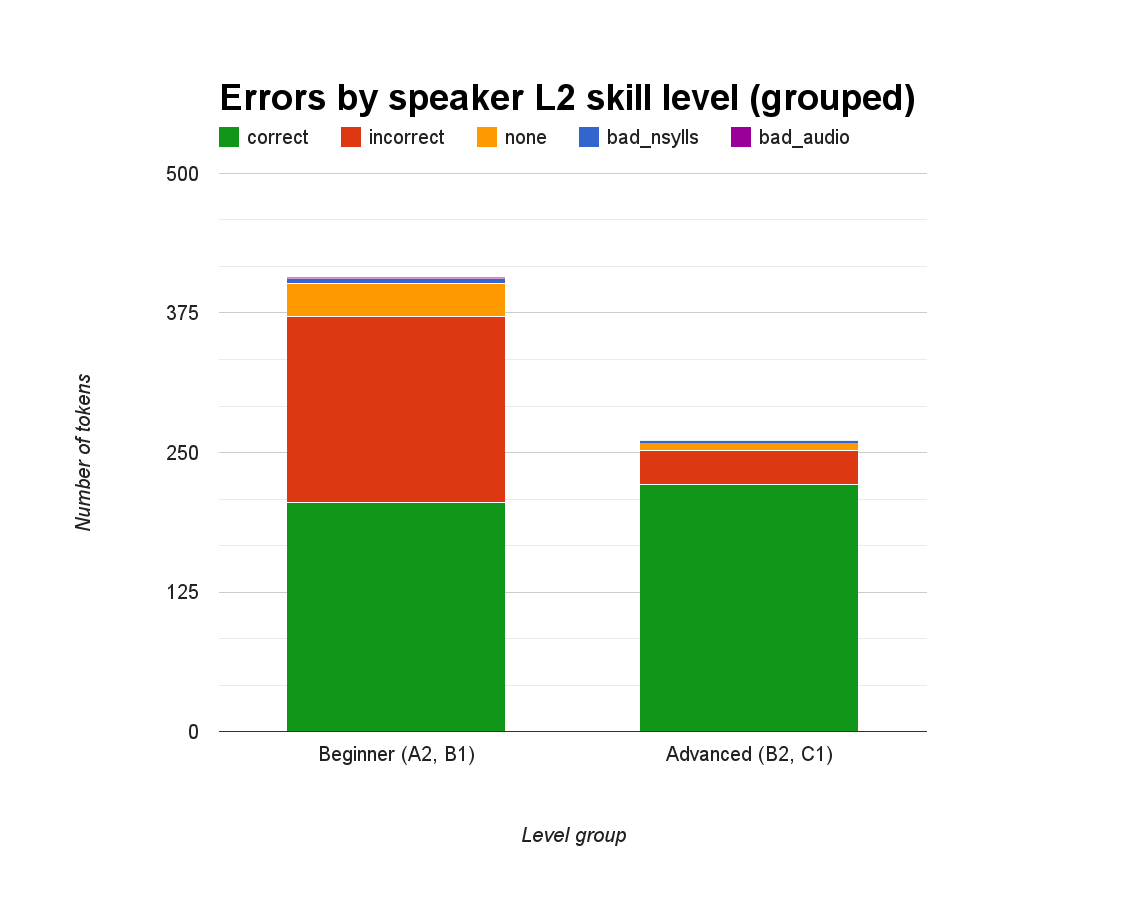
\includegraphics[width=\textwidth]{img/annotation/skillLevelGroupsBars}
				\caption{\TODO{Caption}}
				\label{fig:levelgroupsbars}
			\end{figure}
			
			
			\begin{figure}[htb]
				\centering
				\begin{subfigure}[t]{0.5\textwidth}
					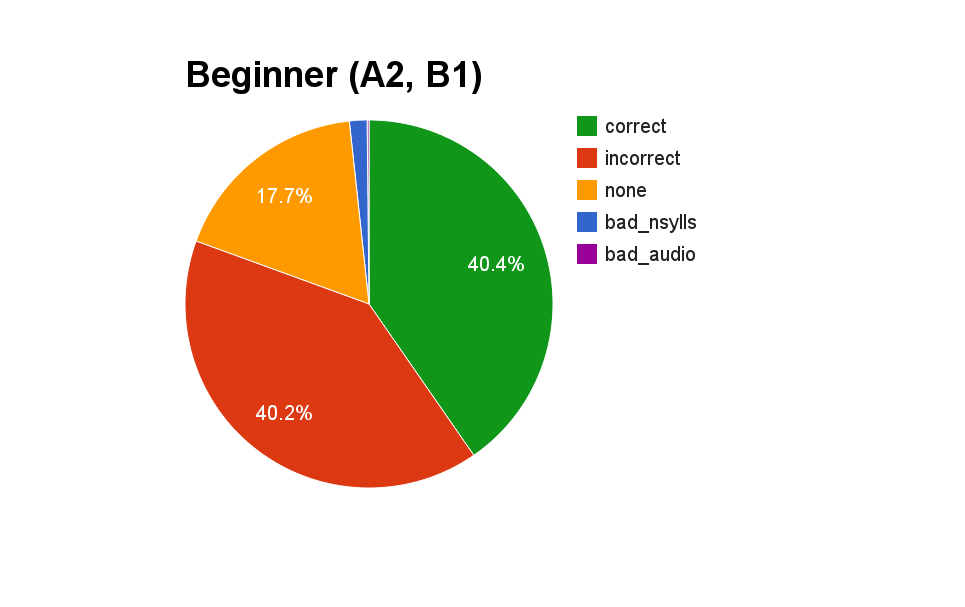
\includegraphics[width=\textwidth]{img/annotation/beginnerPie}
					\caption{}
					\label{fig:levelgroupspies:beg}
				\end{subfigure}%
				~
				\begin{subfigure}[t]{0.5\textwidth}
					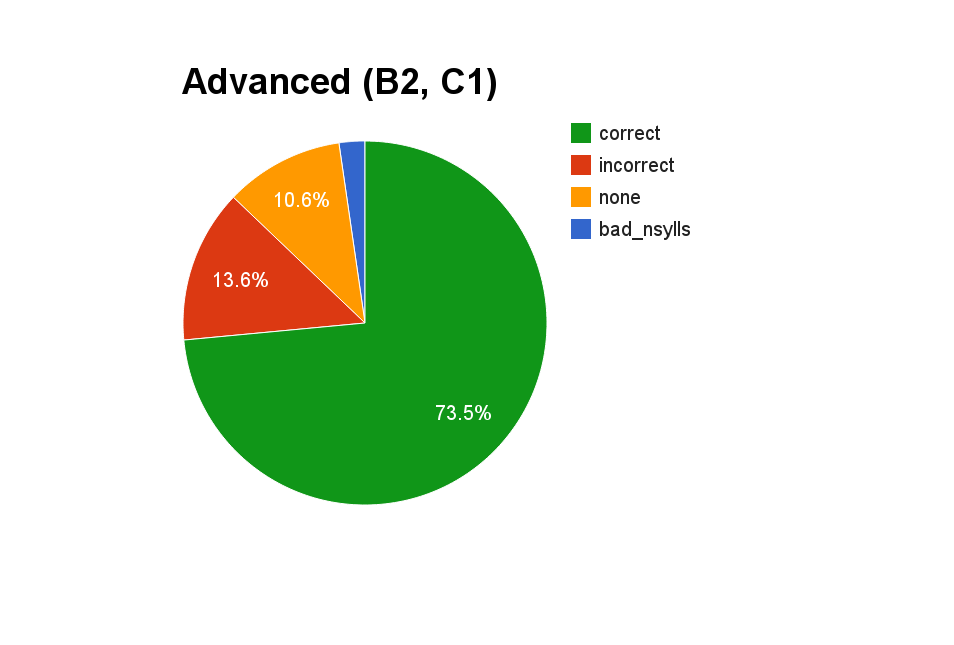
\includegraphics[width=\textwidth]{img/annotation/advancedPie}
					\caption{}
					\label{fig:levelgroupspies:adv}
				\end{subfigure}%
				\caption{\TODO{Caption}}
				\label{fig:levelgroupspies}
			\end{figure}	
			
			
			
		
		\subsection{Errors by recording condition}
		\label{sec:results:condition}
			\TODO{}
		
		
		%\subsubsection{Accuracy by word type}
		\subsection{Errors by word type}
		\label{sec:results:wordtype}
			\TODO{}
	
		\subsection{Impact of technical problems}
		\label{sec:results:techproblems}
			\TODO{}
	
	
	\section{Summary}
	\label{sec:lexstress:summary}
	\TODO{}